\documentclass{standalone}
\usepackage[utf8]{inputenc}
\usepackage{amsmath}
\usepackage{tikz}

\usetikzlibrary{decorations, decorations.pathreplacing, decorations.pathmorphing}

\begin{document}

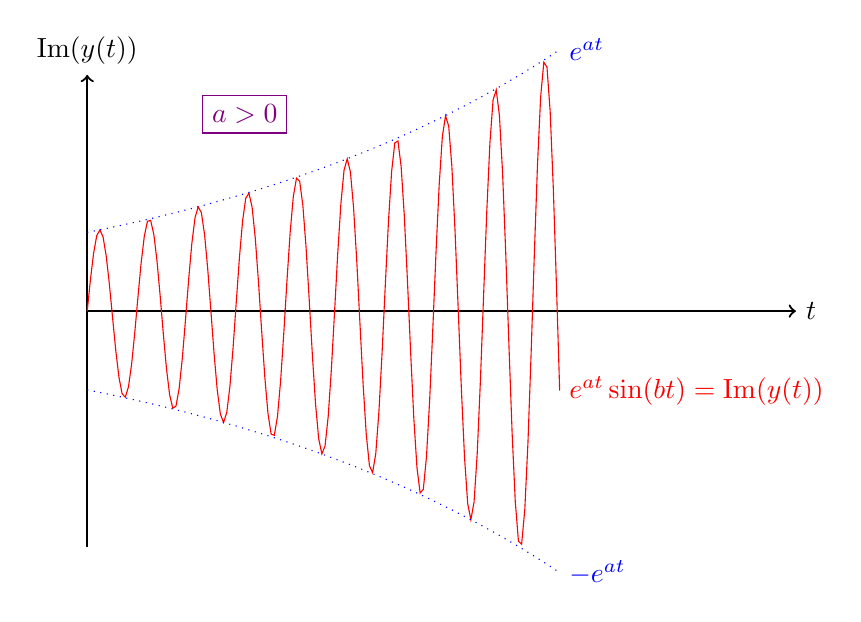
\begin{tikzpicture}[domain=0:6]
    \draw[thick,->] (0,0) -- (9,0) node[right] {$t$};
    \draw[thick,->] (0,-3) -- (0,3) node[above] {Im$(y(t))$};

    \draw[color=red] plot[samples=150](\x,{exp(0.2*\x)*sin(10*\x r)}) node[right] {$e^{at}\sin(bt)=\text{Im}(y(t))$};
    \draw[color=blue, dotted] plot[samples=150](\x,{exp(0.2*\x)}) node[right] {$e^{at}$};
    \draw[color=blue, dotted] plot[samples=150](\x,{-exp(0.2*\x)}) node[right] {$-e^{at}$};
    \node[draw,color=violet] at (2,2.5) {$a>0$};
\end{tikzpicture}

\end{document}
